\section{Construction of the Hermitian Operator \( \hat{H} \)}
Let \( \mathcal{H}_P \) be a Hilbert space spanned by orthonormal basis states \( |p\rangle \), indexed by the first \( N \) primes. Define \( \hat{H} \in \mathbb{R}^{N \times N} \):
\begin{align}
\Hhat_{ij} = \alpha \cdot \frac{\log(p_i p_j)}{\sqrt{p_i p_j}} \cdot \sum_{k=1}^{K} &\cos\left(2\pi \omega_k \log^2(p_i p_j) + \phi_k\right) \nonumber\\
&+ V_{\text{mod}}(p_i \modm)\delta_{ij},
\end{align}
where parameters are listed in Table \ref{tab:parameters}.

\begin{figure}[t]
\centering
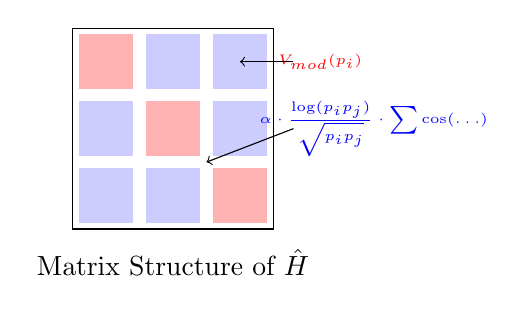
\begin{tikzpicture}[scale=0.85]
    % Draw the operator structure
    % Diagonal elements
    \draw (0,0) rectangle (3,3);
    \foreach \i in {0,...,2} {
        \filldraw[red!30] (\i+0.1,2-\i+0.1) rectangle (\i+0.9,3-\i-0.1);
    }
    
    % Off-diagonal elements
    \foreach \i in {0,...,2} {
        \foreach \j in {0,...,2} {
            \ifnum\i=\j\else
                \filldraw[blue!20] (\i+0.1,2-\j+0.1) rectangle (\i+0.9,3-\j-0.1);
            \fi
        }
    }
    
    % Labels
    \node at (1.5,-0.5) {Matrix Structure of $\hat{H}$};
    \node[red] at (3.7,2.5) {\tiny $V_{\text{mod}}(p_i \modm)$};
    \node[blue] at (4.5,1.5) {\tiny $\alpha \cdot \frac{\log(p_i p_j)}{\sqrt{p_i p_j}} \cdot \sum \cos(\ldots)$};
    
    % Draw arrows to elements
    \draw[->] (3.3,2.5) -- (2.5,2.5);
    \draw[->] (3.3,1.5) -- (2.0,1.0);
\end{tikzpicture}
\caption{Structure of the Hermitian operator $\hat{H}$, showing diagonal elements (red) containing the modular potential and off-diagonal elements (blue) encoding prime interactions.}
\label{fig:operator_structure}
\end{figure}

\begin{figure*}[t]
\centering
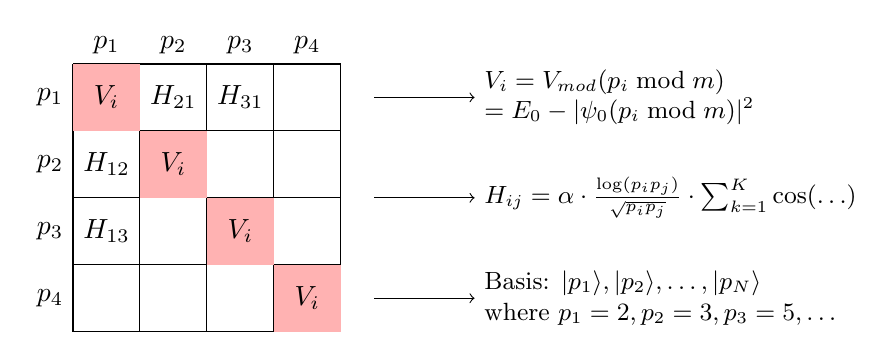
\begin{tikzpicture}[scale=0.85]
    % Create a more detailed visualization of operator components
    % Draw a sample 4×4 matrix
    \draw (0,0) grid (4,4);
    
    % Highlight diagonal elements
    \foreach \i in {0,...,3} {
        \fill[red!30] (\i,3-\i) rectangle (\i+1,4-\i);
        \node at (\i+0.5,3.5-\i) {$V_i$};
    }
    
    % Example off-diagonal elements with values
    \node at (0.5,2.5) {$H_{12}$};
    \node at (1.5,3.5) {$H_{21}$};
    \node at (0.5,1.5) {$H_{13}$};
    \node at (2.5,3.5) {$H_{31}$};
    
    % Add matrix labels
    \node[left] at (0,3.5) {$p_1$};
    \node[left] at (0,2.5) {$p_2$};
    \node[left] at (0,1.5) {$p_3$};
    \node[left] at (0,0.5) {$p_4$};
    
    \node[above] at (0.5,4) {$p_1$};
    \node[above] at (1.5,4) {$p_2$};
    \node[above] at (2.5,4) {$p_3$};
    \node[above] at (3.5,4) {$p_4$};
    
    % Add formulas and components
    \draw[->] (4.5,3.5) -- (6,3.5);
    \node[align=left, anchor=west, font=\small] at (6,3.5) {$V_i = V_{\text{mod}}(p_i \bmod m)$\\$= E_0 - |\psi_0(p_i \bmod m)|^2$};
    
    \draw[->] (4.5,2) -- (6,2);
    \node[align=left, anchor=west, font=\small] at (6,2) {$H_{ij} = \alpha \cdot \frac{\log(p_i p_j)}{\sqrt{p_i p_j}} \cdot \sum_{k=1}^{K} \cos(\ldots)$};
    
    % Prime basis illustration
    \draw[->] (4.5,0.5) -- (6,0.5);
    \node[align=left, anchor=west, font=\small] at (6,0.5) {Basis: $|p_1\rangle, |p_2\rangle, \ldots, |p_N\rangle$\\where $p_1=2, p_2=3, p_3=5, \ldots$};
\end{tikzpicture}
\caption{Detailed construction of the Hermitian operator $\hat{H}$. Diagonal elements (red) contain the modular potential values $V_{\text{mod}}(p_i \bmod m)$, while off-diagonal elements encode prime interactions through the logarithmic cosine terms. The matrix acts on a Hilbert space with prime-indexed basis states.}
\label{fig:operator_detailed}
\end{figure*}

\begin{table}[t]
\centering
\small
\begin{tabular}{|c|c|}
\hline
\textbf{Parameter} & \textbf{Value} \\ \hline
\( \alpha \) & 0.01 \\ \hline
\( \omega_k \) & \( k/10 \), \( k = 1, 2, 3 \) \\ \hline
\( \phi_k \) & 0 \\ \hline
\( K \) & 3 \\ \hline
\end{tabular}
\caption{Parameter values for \( \hat{H} \).}
\label{tab:parameters}
\end{table}

% TODO: Conduct sensitivity analysis for parameters \alpha, \omega_k, \phi_k, K.
% TODO: Provide theoretical justification for parameter choices if possible.
% The current parameters appear empirically tuned; robustness needs verification.

\subsection*{Theoretical Motivation for Off-Diagonal Terms}
The off-diagonal terms:
\[
\frac{\log(p_i p_j)}{\sqrt{p_i p_j}} \sum_{k=1}^{K} \cos\left(2\pi \omega_k \log^2(p_i p_j) + \phi_k\right)
\]
are inspired by the logarithmic derivative of \(\zs\):
\[
-\frac{\zeta'(s)}{\zeta(s)} = \sum_p \sum_{k=1}^\infty \frac{\log p}{p^{ks}}.
\]
The term \( \log(p_i p_j) \) captures prime interactions, and \( \sqrt{p_i p_j} \) normalizes magnitude. The cosine modulation with \( \log^2(p_i p_j) \) approximates oscillations in the prime number theorem's error term, as seen in Montgomery's pair correlation \cite{Montgomery1973}. This structure aims to encode the zeta function's analytic behavior spectrally.